
Cho tập $ I = \{i_1, i_2, ..., i_m\}$ là tập các món hàng (item) khác nhau. Một giao dịch (transaction) $T_j = \{x_l | 1, 2, ...N_j, x_l \in I \} $ với $N_j$ là số hàng trong giao dịch  $T_j$. Một cơ sở dữ liệu (database) $D$ có chứa các giao dịch, $D = \{T_1, T_2, ..., T_m\}$, với $m$ số các giao dịch trong cơ sở dữ liệu. Một tập hợp chưa các món hàng $X =\{ x_1, x_2, ... x_k \} \subset I, x_i \in I $ gọi là k-itemset. 

Hình \ref{fig:table2} là một cơ sở dữ liệu D chứa thông tin các giao dịchụ. Hình \ref{fig:table3} là lợi nhuận mỗi đơn vị của mỗi món hàng, và giá trị sử dụng tối thiểu được cho trước.



\begin{figure}[h]
\centering
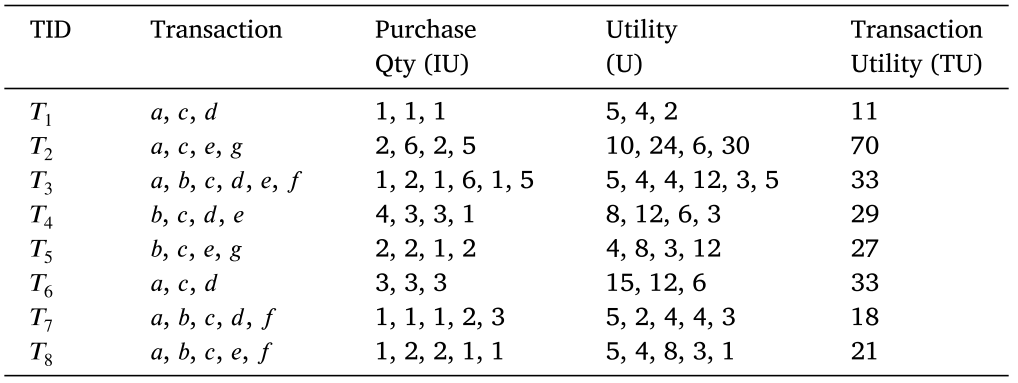
\includegraphics[width=0.9\textwidth]{image/table/table2.PNG}
\caption{\label{fig:table2} Cơ sở dữ liệu}
\end{figure}

\begin{figure}[h]
\centering
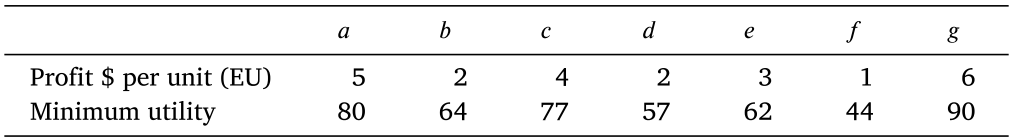
\includegraphics[width=0.9\textwidth]{image/table/table3.PNG}
\caption{\label{fig:table3} Lợi nhuận và giá trị sử dụng tối thiểu}
\end{figure}

\paragraph{Định nghĩa 1}: $ MU(x_i) $ là giá trị tiện ít tối thiểu (minimum utility threshold) của món hàng $x_i$. Thực tế, giá trị tiện ích tối thiểu của món hàng thể hiện hạn mức quan trọng của người dùng đối với món hàng đó. Trong quá trình khai thác, ta tính giá trị tiện ích của mỗi món hàng. Nếu giá trị tiện ích dưới giá trị tiện ích tối thiểu, ta không xét món hàng đó nữa. 

\paragraph{Định nghĩa 2} $MIU(X)$ là giá trị tiện ích tối thiểu của k-itemset, là $MU(x)$ với $x$ là món hàng có giá trị tiện ích tối thiểu nhỏ nhất. $MIU(X) = min \{MU(x_j|x_j \in X\}$ . Ví dụ: $MIU(a) = 80$, $MIU(af) = min\{MU(a), MU(f)\} = 44$


\paragraph{Định nghĩa 3} Chỉ số support của itemset X trong cơ sở dữ liệu D kí hiệu là $Sup(X)$. Support của itemset là tỉ lệ của tần số xuất hiện của itemsetX và tổng số giao dịch n. Ví dụ: $Sup(ac) = 6/8$

\paragraph{Định nghĩa 4} Mỗi món hàng $x_i \in I$ đều có giá trị tiện ích ngoài (external utility value), ký hiệu là $EU(x_i)$. Ví dụ: trong hình \ref{fig:table3} $EU(b) = 2$

\paragraph{Định nghĩa 5} Mỗi món hàng $x_i \in T_j$ có giá trị tiện ích bên trong (internal utility value), kí hiệu là $IU(x_i, T_j)$. Ví dụ: trong hình \ref{fig:table2}, $UI(b, T_3) = 2$

\paragraph{Định nghĩa 6} Giá trị tiện ích của món hàng $x_i \in T_j$ kí hiệu $U(x_i, T_j)$ là tích của giá trị tiện ích ngoài và giá trị tiện ích bên trong. 

$$ U(x_i, T_j) = EU(x_i) \times IU(x_i, T_j) $$ .

Ví dụ: $U(b, T_3) = EU(b) \times IU(b, T_3) = 2 \times 2 = 4$

Giá trị tiện ích thể hiện mức độ quan trọng của món hàng về số lượng được mua (giá trị tiện ích trong) và lợi nhuận mỗi đơn vị (giá trị tiện ích ngoài)

\paragraph{Định nghĩa 7} Giá trị tiện ích của itemset X trong giao dịch $T_j$ là tổng giá trị tiện ích của mỗi món hàng trong itemset đó. 
$$U(X, T_j) = \sum_{x_i \in X} U(x_i, T_j)$$
Ví dụ: trong hình \ref{fig:table2}, $U(ac, T_1) = 5 + 4 = 9$

\paragraph{Định nghĩa 8} $U(X)$ giá trị tiện ích của itemset X trong cơ sở dữ liệu D, bằng tổng giá trị tiện ích của itemset X trong mỗi giao dịch $T_j$

$$ U(X) = \sum_{x_i \subseteq T_j \in D} U(X, T_j) $$

Ví dụ: $U(ac) = U(ac, T_1) + U(ac, T_2) + U(ac, T_3) + U(ac, T_6) + U(ac, T_7) + U(ac, T_8) = 9 + 34 + 9 + 28 + 9 + 13 = 101 $

\paragraph{Định nghĩa 9} Tiện ích của giao dịch $TU(T_j)$ là tổng tiện ích của mỗi món hàng trong giao dịch j.

$$ TU(T_j) = \sum_{X \subseteq T_j and x_i \in X} U(x_i, T_j) $$

Ví dụ: $TU(T_5) = U(b, T_5) + U(c, T_5) + U(e, T_5) + U(g, T_5) = 27$

\paragraph{Định nghĩa 10}  $TWU(X)$ là trọng số giao dịch tiện ích (transaction weighted utility) của itemset X , bằng tổng tiện ích của các giao dịch có chứa itemset X.

$$ TWU(X) = \sum_{X \subseteq T_j \in D} TU(T_j) $$

Giá trị $TWU$ của từng món hàng ghi trong hình \ref{fig:table4}.



\begin{figure}[h]
\centering
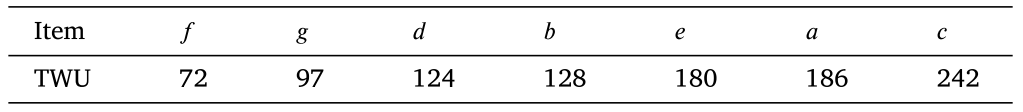
\includegraphics[width=0.9\textwidth]{image/table/table4.PNG}
\caption{\label{fig:table4} Trọng số giao dịch tiện ích  }
\end{figure}

\paragraph{Định nghĩa 11} $T_j/X$ là tập hợp các món hàng sau $X$ trong $T_j$. Ví dụ: trong hình \ref{fig:table2}, $T_i/ac = d, T_7/ac = df$.

\paragraph{Định nghĩa 12} $RU(X, T_j)$  là tiện ích còn lại (remaining utility) của itemset X trong giao dịch $T_j(X \subseteq T_j)$.

$$ RU(X, T_j) = \sum_{x_i \in (T_j/X)} U(x_i, T_j) $$

Ví dụ, trong hình \ref{fig:table2}, $RU(ac, T_1) = 2, RU(ac, T_7) = 4 + 3 = 7 $  

\paragraph{Định nghĩa 13} $RU(X)$ là tiện ích còn lại của itemset X trong cơ sở dữ liệu D, tính bằng tổng các tiện ích còn lại của X ở mỗi giao dịch $T_j$

$$ RU(X) = \sum_{X \subseteq T_j \in D} RU(x, T_j) $$

Ví dụ, trong hình \ref{fig:table2}, $RU(ac) = 2 + 36 + 20 + 6 + 7 + 4 = 75$

\paragraph{Định nghĩa 14} (Về thứ tự các món hàng). Các món hàng trong cơ sở dữ liệu các giao dịch được xử lý theo thứ tự $\succ$ xếp theo giá trị TWU tăng dần. Trong ví dụ của bài báo thứ tự là $ f \succ g \succ d \succ b \succ e \succ a \succ c $. Hình \ref{fig:table5} là cơ sở dữ liệu với mỗi giao dịch đã được sắp xếp các món hàng theo thứ tự TWU. 

\begin{figure}[h]
\centering
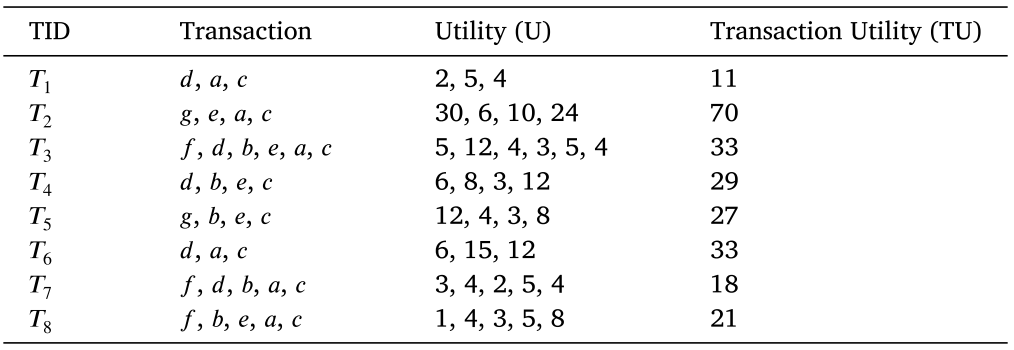
\includegraphics[width=0.9\textwidth]{image/table/table5.PNG}
\caption{\label{fig:table5} Cơ sở dữ liệu sau khi sắp xếp theo TWU  }
\end{figure}

\paragraph{Định nghĩa 15} (Về phần mở rộng của itemset). $Ext(X)$ là phần mở rộng của itemset X, là tất cả các món hàng sau X trong tập hợp các món hàng được xếp theo thứ tự. Ví dụ: $Ext(b) = \{ e, a, c \}$ và $Ext(fd) = \{b, e, a, c \}$.

\paragraph{Định nghĩa 16} $SMU(X)$ là hậu tố tiện ích tối thiểu (suffix minimum utility) của X. 

$$ SMU(U) = min(MIU(X), MIU(Ext(X))) $$

Ví dụ, $SMU(ea) = min(MIU(ea), MIU(Ext(ea))) = min (MIU(ea), MIU(c)) = min(min(62, 80), 77) = 62$

\paragraph{Định nghĩa 17} EUCS, cấu trúc đồng xảy ra tiện ích ước tính (Estimated Utility Co-occurrence Structure) \cite{fournier2014fhm} là một ma trận tam giác như hình \ref{fig:eucs}. Ma trận này để chứa giá trị TWU của một cặp itemset. $EUCS(x_i, x_j) = TWU(x_i) + TWU(x_j)$

\begin{figure}[h]
\centering
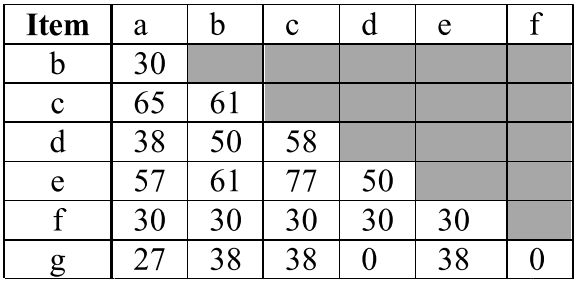
\includegraphics[width=0.7\textwidth]{image/fig/trianglematrix.PNG}
\caption{\label{fig:eucs} Ma trận tam giác  }
\end{figure}